\documentclass[border=10pt]{standalone}
\usepackage{tikz}
\usetikzlibrary{arrows.meta, positioning, calc}
\usepackage{xcolor}
\usepackage{amsmath}

% Brand colors
\definecolor{Congaree}{HTML}{1F414D}
\definecolor{Atlantic}{HTML}{466A9F}
\definecolor{Horseshoe}{HTML}{65780B}
\definecolor{Rose}{HTML}{CC2E40}
\definecolor{LightGray}{HTML}{ECECEC}
\definecolor{WarmGrey}{HTML}{676156}

\begin{document}
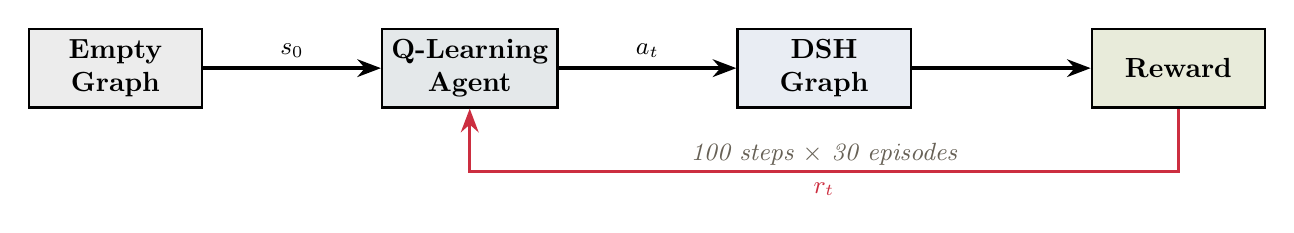
\begin{tikzpicture}[
    block/.style={draw, thick, minimum width=2.2cm, minimum height=1.0cm,
        align=center, font=\normalsize\bfseries},
    arr/.style={-{Stealth[length=3mm]}, very thick},
    every node/.style={font=\normalsize}
]

\node[block, fill=LightGray] (empty) at (0, 0) {Empty\\Graph};
\node[block, fill=Congaree!12] (agent) at (4.5, 0) {Q-Learning\\Agent};
\node[block, fill=Atlantic!12] (graph) at (9.0, 0) {DSH\\Graph};
\node[block, fill=Horseshoe!15] (reward) at (13.5, 0) {Reward};

\draw[arr] (empty.east) -- (agent.west) node[midway, above, font=\small] {$s_0$};
\draw[arr] (agent.east) -- (graph.west) node[midway, above, font=\small] {$a_t$};
\draw[arr] (graph.east) -- (reward.west);
\draw[arr, Rose] (reward.south) -- ++(0,-0.8) -| (agent.south)
    node[pos=0.25, below, font=\small, text=Rose] {$r_t$};

\node[font=\small\itshape, WarmGrey] at (9.0, -1.1) {100 steps $\times$ 30 episodes};

\end{tikzpicture}
\end{document}
